\chapter{Les transformations sans retour}\label{ch:g5:irreversible-changes}

On casse un œuf dans une poêle chaude. En quelques secondes, le blanc
transparent et coulant devient ferme et blanc, et le jaune épaissit.
Retire la poêle du feu, laisse refroidir l'œuf, mets-le au
réfrigérateur~: il ne redeviendra jamais un œuf cru. Certaines
transformations peuvent être défaites, d'autres non. Savoir les
distinguer, c'est le premier pas de la chimie.

\begin{recall}
Un solide qui \omterm{def:g2:mixing-and-dissolving:dissolve}{se dissout} dans l'eau est toujours là~: quand l'eau sèche,
le solide reste (\cref{ch:g2:mixing-and-dissolving}). Une \omterm{def:g4:what-a-fire-needs:burning}{combustion}
fabrique de nouvelles substances --- cendre, fumée, dioxyde de carbone,
vapeur d'eau --- et le \omterm{def:g4:what-a-fire-needs:fuel}{combustible} a disparu pour de bon
(\cref{ch:g4:what-a-fire-needs}).
\end{recall}

\begin{omfigure}
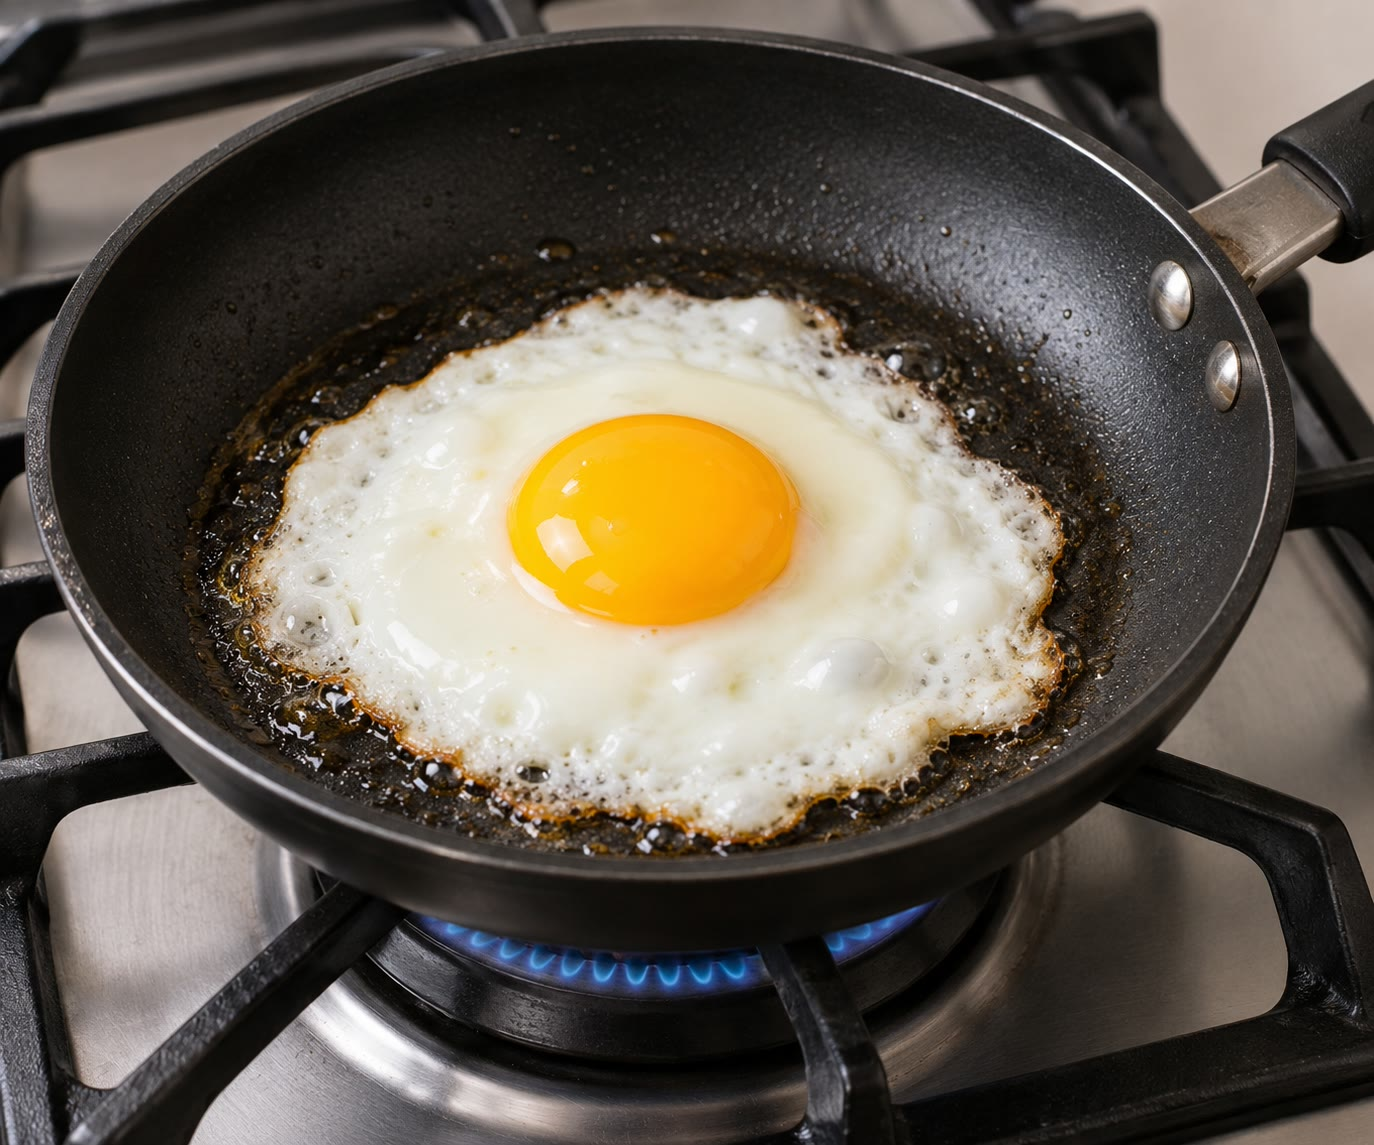
\includegraphics[width=0.55\linewidth]{images/book1/ai/g5-egg-frying.jpg}

{\small Un œuf au plat~: le blanc transparent est devenu ferme et blanc,
pour de bon.}
\end{omfigure}

\section{Les transformations que l'on peut défaire}

\begin{definition}[Transformation réversible]\label{def:g5:irreversible-changes:reversible}
Une \emph{transformation réversible}\index{transformation reversible@transformation réversible} est
une transformation que l'on peut défaire, de façon à retrouver
exactement ce que l'on avait au départ.
\end{definition}

\begin{example}[Dissoudre puis faire sécher]\label{ex:g5:irreversible-changes:dissolve}
Du sucre remué dans l'eau \omterm{def:g2:mixing-and-dissolving:dissolve}{se dissout}. Laisse l'eau s'évaporer, et le
sucre revient~: le même sucre, aussi sucré qu'avant. La dissolution est
une \omterm{def:g5:irreversible-changes:reversible}{transformation réversible}.
\end{example}

\begin{example}[La glace et l'eau]\label{ex:g5:irreversible-changes:ice}
Un glaçon fond en eau sur une assiette tiède~; mets l'eau au congélateur
et elle redevient de la glace. La fusion et la solidification sont des
\omterm{def:g5:irreversible-changes:reversible}{transformations réversibles}. (Pourquoi l'eau fond et gèle, c'est le
livre de physique qui l'explique.)
\end{example}

\begin{example}[Mélanger]\label{ex:g5:irreversible-changes:mix}
Du sable mélangé à du gravier peut être de nouveau séparé au tamis~; une
eau boueuse peut être filtrée. \omterm{def:g2:mixing-and-dissolving:mix}{Mélanger} est une \omterm{def:g5:irreversible-changes:reversible}{transformation
réversible}~: rien de nouveau n'est fabriqué, et les parties peuvent être
séparées (\cref{ch:g3:separating-mixtures}).
\end{example}

\section{Les transformations que l'on ne peut pas défaire}

\begin{definition}[Transformation irréversible et transformation chimique]\label{def:g5:irreversible-changes:chemical-change}
Une \emph{transformation irréversible}\index{transformation irreversible@transformation irréversible}
est une transformation que l'on ne peut pas défaire simplement. La
plupart sont des transformations au cours desquelles apparaissent de
nouvelles substances qui n'étaient pas là au départ~: une telle
transformation s'appelle une
\emph{transformation chimique}\index{transformation chimique}.
\end{definition}

\begin{example}[Six transformations chimiques]\label{ex:g5:irreversible-changes:six}
\begin{itemize}
  \item \textbf{Faire cuire un œuf}~: le blanc coulant et transparent
        devient ferme et blanc.
  \item \textbf{Faire cuire un gâteau}~: une pâte liquide devient un
        gâteau moelleux, doré à l'extérieur, avec une odeur nouvelle.
  \item \textbf{\omterm{def:g4:what-a-fire-needs:burning}{Brûler}}~: le bois devient cendre, fumée, dioxyde de
        carbone et vapeur d'eau.
  \item \textbf{Rouiller}~: du fer brillant laissé sous la pluie se
        couvre d'une substance orange-brun qui s'écaille, la rouille.
  \item \textbf{Le lait qui tourne}~: oublié plusieurs jours, le lait
        épaissit, forme des grumeaux et sent l'aigre.
  \item \textbf{Une pomme coupée qui brunit}~: sa chair claire devient
        brune à l'\omterm{def:g4:air-a-mixture-of-gases:air}{air} en moins d'une heure.
\end{itemize}
Dans chaque cas, quelque chose de nouveau a été fabriqué, et il n'existe
aucun moyen simple de retrouver ce que l'on avait au départ.
\end{example}

\begin{omfigure}
\begin{minipage}[t]{0.48\linewidth}\centering
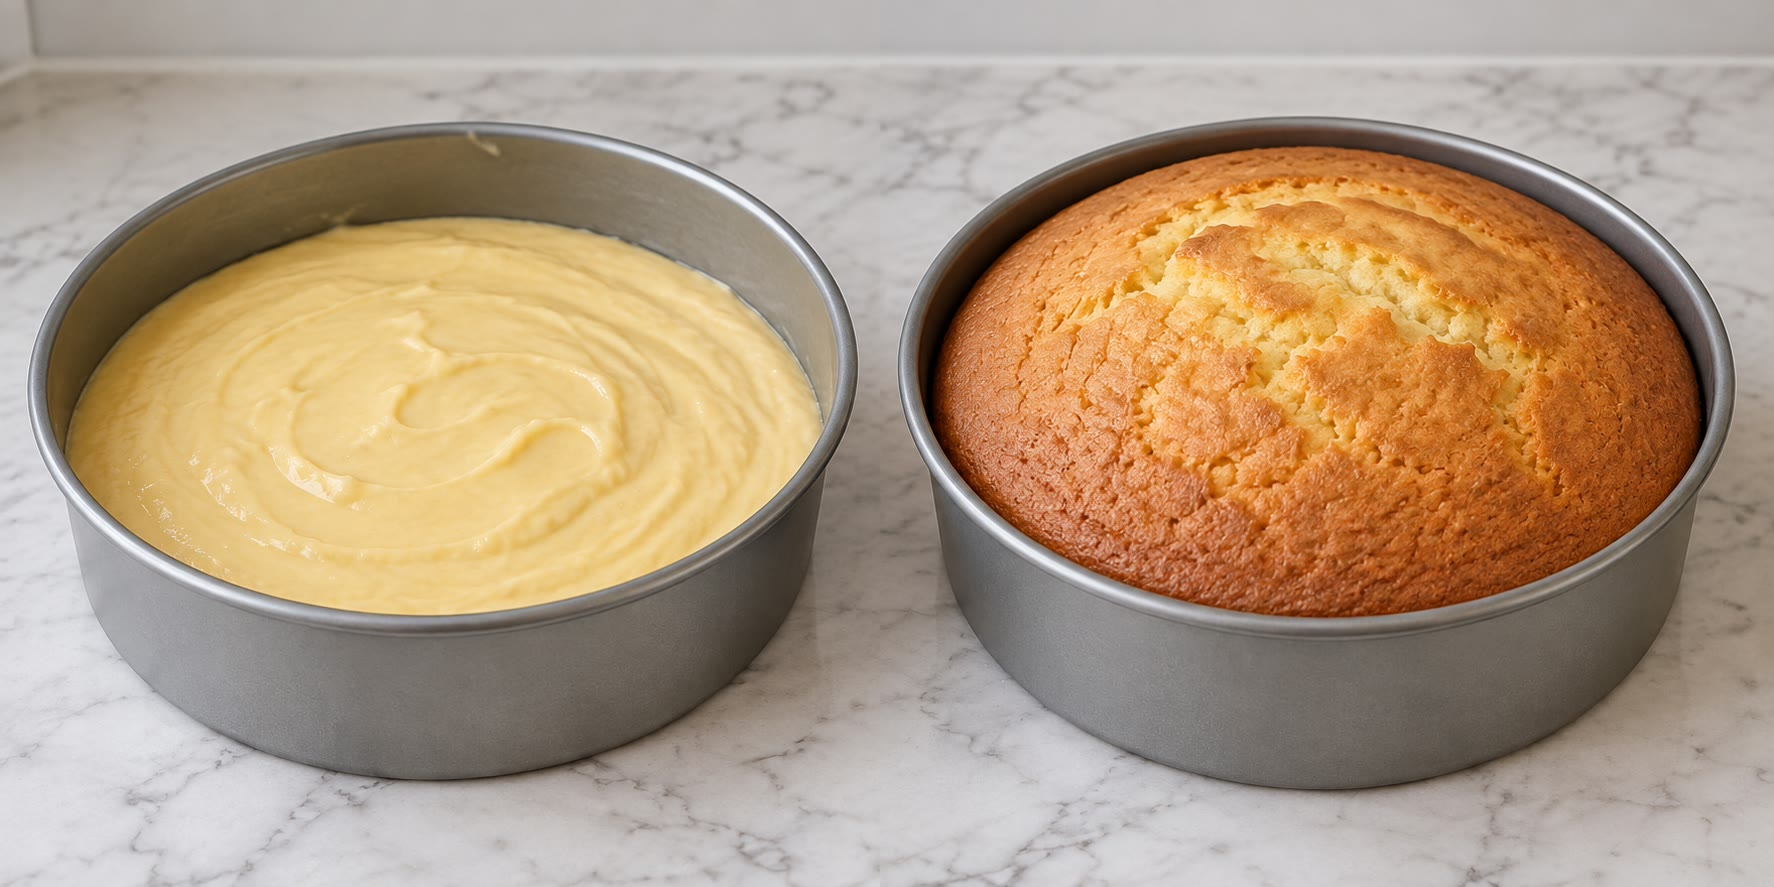
\includegraphics[width=\linewidth,height=4.6cm,keepaspectratio]{images/book1/ai/g5-cake-before-after.jpg}

{\small La pâte avant, le gâteau après~: la cuisson ne peut pas être
défaite.}
\end{minipage}\hfill
\begin{minipage}[t]{0.48\linewidth}\centering
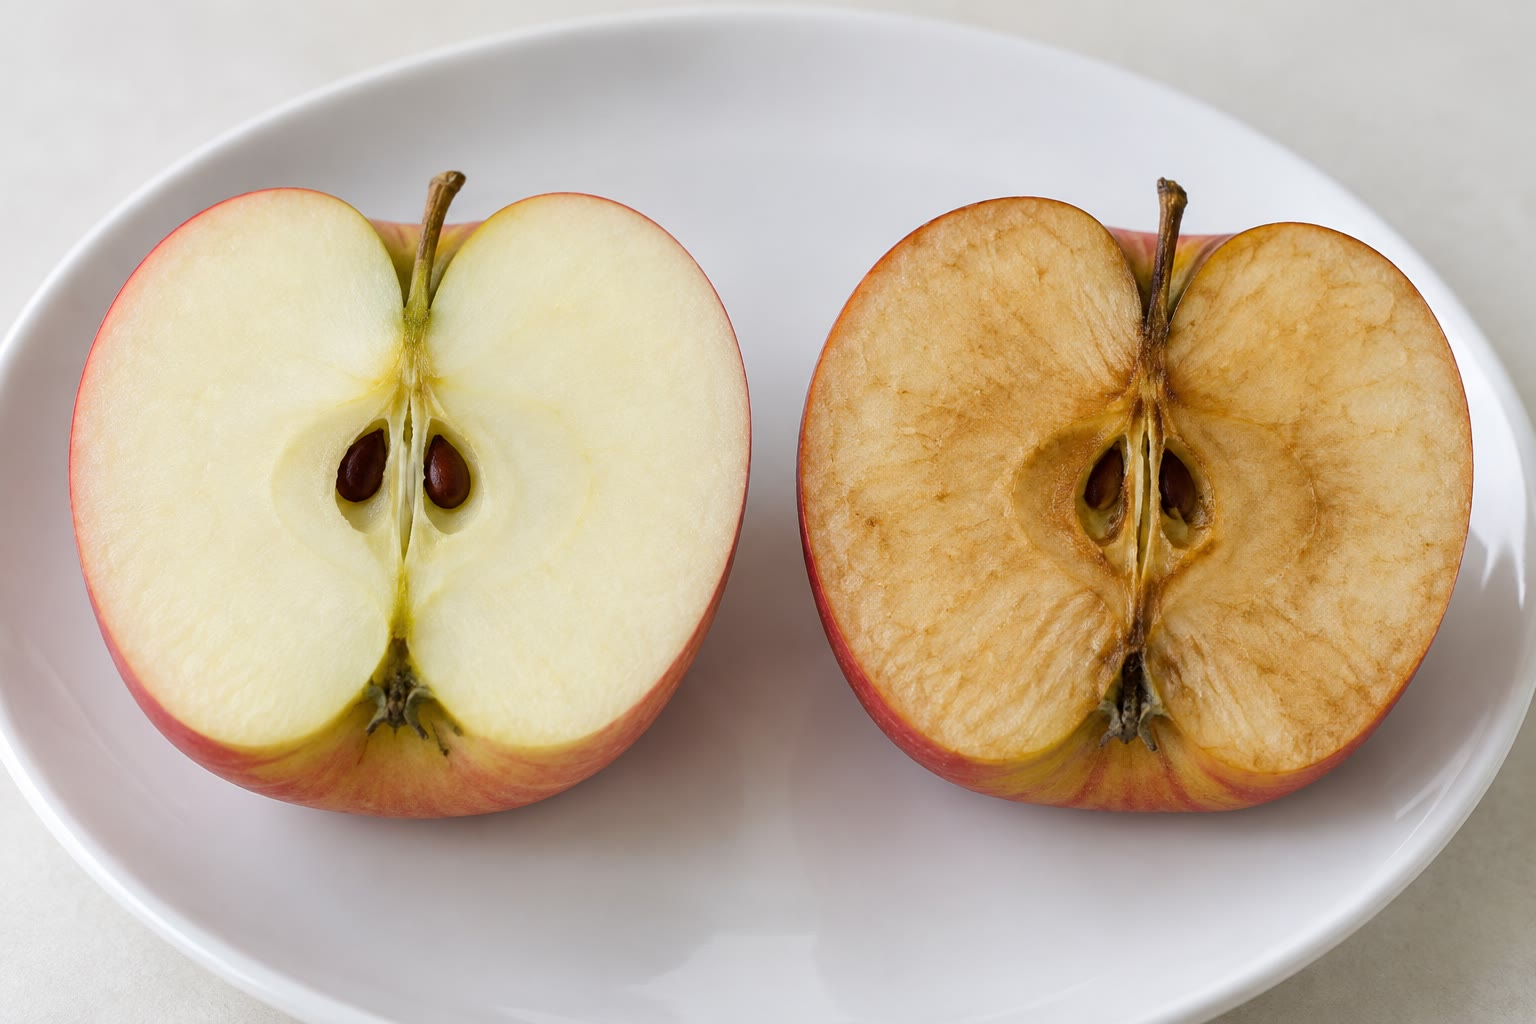
\includegraphics[width=\linewidth,height=4.6cm,keepaspectratio]{images/book1/ai/g5-apple-browning.jpg}

{\small Une moitié fraîche, et une moitié laissée une heure à l'\omterm{def:g4:air-a-mixture-of-gases:air}{air}.}
\end{minipage}
\end{omfigure}

\begin{omfigure}
\begin{tikzpicture}[font=\small]
  \node[font=\small\bfseries, omDef] at (2.7,4.6) {peut être défaite};
  \node[font=\small\bfseries, omProp] at (9.6,4.6) {ne peut pas être défaite};
  \draw[black!30] (6.1,4.9) -- (6.1,-0.3);
  % reversible pairs
  \foreach \y/\a/\b in {3.6/{sucre + eau}/{eau sucrée}, 2.0/{glace}/{eau liquide},
                        0.4/{sable + gravier}/{un mélange}} {
    \node[draw=omDef, fill=omDef!6, rounded corners=2pt, minimum width=2.3cm,
      minimum height=0.8cm] at (0.9,\y) {\a};
    \node[draw=omDef, fill=omDef!6, rounded corners=2pt, minimum width=2.3cm,
      minimum height=0.8cm] at (4.6,\y) {\b};
    \draw[->, thick, omDef] (2.3,\y+0.12) -- (3.25,\y+0.12);
    \draw[<-, thick, omDef] (2.3,\y-0.12) -- (3.25,\y-0.12);
  }
  % irreversible ones
  \foreach \y/\a/\b in {3.6/{œuf cru}/{œuf cuit}, 2.0/{bois}/{cendre, fumée, gaz},
                        0.4/{fer}/{rouille}} {
    \node[draw=omProp, fill=omProp!6, rounded corners=2pt, minimum width=2.0cm,
      minimum height=0.8cm] at (7.6,\y) {\a};
    \node[draw=omProp, fill=omProp!6, rounded corners=2pt, minimum width=2.9cm,
      minimum height=0.8cm] at (11.5,\y) {\b};
    \draw[->, thick, omProp] (8.8,\y) -- (9.85,\y);
  }
\end{tikzpicture}

{\small À gauche~: des \omterm{def:g5:irreversible-changes:reversible}{transformations réversibles}, la double flèche
indique qu'elles peuvent aller dans les deux sens. À droite~: des
\omterm{def:g5:irreversible-changes:chemical-change}{transformations chimiques}, dans un seul sens.}
\end{omfigure}

\section{Les indices de l'apparition d'une nouvelle substance}

\begin{method}[Est-ce une transformation chimique~? Cherche les indices]\label{met:g5:irreversible-changes:clues}
Une nouvelle substance se trahit souvent par l'un de ces indices~:
\begin{enumerate}
  \item une nouvelle \textbf{couleur} (le brun d'une tranche de pain
        grillé)~;
  \item des \textbf{bulles} de gaz qui apparaissent dans un liquide sans
        qu'on le chauffe (du vinaigre versé sur du bicarbonate de
        soude)~;
  \item une nouvelle \textbf{odeur} (le lait tourné, le pain brûlé)~;
  \item de la \textbf{chaleur ou de la lumière} dégagée (une bougie
        allumée)~;
  \item un \textbf{solide qui apparaît} dans un liquide limpide, ou des
        grumeaux qui se forment (le lait qui caille).
\end{enumerate}
Un seul indice peut tromper~: l'eau qui bout fait des bulles, mais rien
de nouveau n'est fabriqué --- les bulles sont de la vapeur d'eau, et
l'eau revient quand la vapeur refroidit. Cherche plusieurs indices, et
demande-toi~: peut-on la défaire~?
\end{method}

\begin{omfigure}
\begin{tikzpicture}[font=\small]
  \foreach \k/\t in {0/{nouvelle couleur}, 1/{bulles de gaz}, 2/{nouvelle odeur},
                     3/{chaleur ou lumière}, 4/{un solide apparaît}} {
    \begin{scope}[xshift=\k*3.2cm]
      \draw[omProp, line width=0.8pt, fill=omProp!5] (0,0) circle (1.0);
      \node[anchor=north, align=center] at (0,-1.15) {\t};
    \end{scope}
  }
  % 1: colour, a slice of toast half brown
  \fill[yellow!20, draw=brown!60] (-0.55,-0.5) rectangle (0.55,0.55);
  \fill[brown!55] (0,-0.5) rectangle (0.55,0.55);
  % 2: bubbles in a beaker
  \begin{scope}[xshift=3.2cm]
    \pic[transform shape, scale=0.45] at (0,-0.55) {beaker={0.7}{omWater!80}};
    \foreach \x/\y in {-0.15/-0.2,0.1/0.05,-0.05/0.25,0.18/-0.35,-0.2/0.15}
      \draw[black!55] (\x,\y) circle (0.05);
  \end{scope}
  % 3: smell, wavy lines
  \begin{scope}[xshift=6.4cm]
    \foreach \x in {-0.35,0,0.35} \draw[black!55, line width=0.8pt, decorate,
      decoration={snake, amplitude=1.5pt, segment length=6pt}] (\x,-0.6) -- (\x,0.6);
  \end{scope}
  % 4: a flame
  \begin{scope}[xshift=9.6cm]
    \fill[orange!80] (0,-0.6) .. controls (-0.45,-0.05) and (-0.15,0.35) .. (0,0.7)
      .. controls (0.15,0.35) and (0.45,-0.05) .. (0,-0.6);
    \fill[yellow!80] (0,-0.45) .. controls (-0.2,-0.1) and (-0.08,0.15) .. (0,0.3)
      .. controls (0.08,0.15) and (0.2,-0.1) .. (0,-0.45);
  \end{scope}
  % 5: solid settling in a test tube
  \begin{scope}[xshift=12.8cm]
    \pic[transform shape, scale=0.4] at (0,-0.65) {testtube={0.75}{omWater!80}};
    \fill[white, draw=black!40] (-0.08,-0.62) rectangle (0.08,-0.5);
    \foreach \x/\y in {-0.04/-0.3,0.04/-0.1,0/0.1} \fill[black!35] (\x,\y) circle (0.03);
  \end{scope}
\end{tikzpicture}

{\small Cinq indices qu'une \omterm{def:g5:irreversible-changes:chemical-change}{transformation chimique} a pu avoir lieu.}
\end{omfigure}

\begin{inthelab}[Du vinaigre sur du bicarbonate]
L'enseignant met une cuillerée de bicarbonate de soude, une poudre
blanche, au fond d'un bécher et y verse un peu de vinaigre. Le \omterm{def:g2:mixing-and-dissolving:mix}{mélange}
pétille et mousse aussitôt~: un gaz se dégage, indice d'une
\omterm{def:g5:irreversible-changes:chemical-change}{transformation chimique}. Quand l'effervescence s'arrête, le bicarbonate
a disparu, et on ne peut pas le récupérer en faisant sécher.
\end{inthelab}

\begin{omfigure}
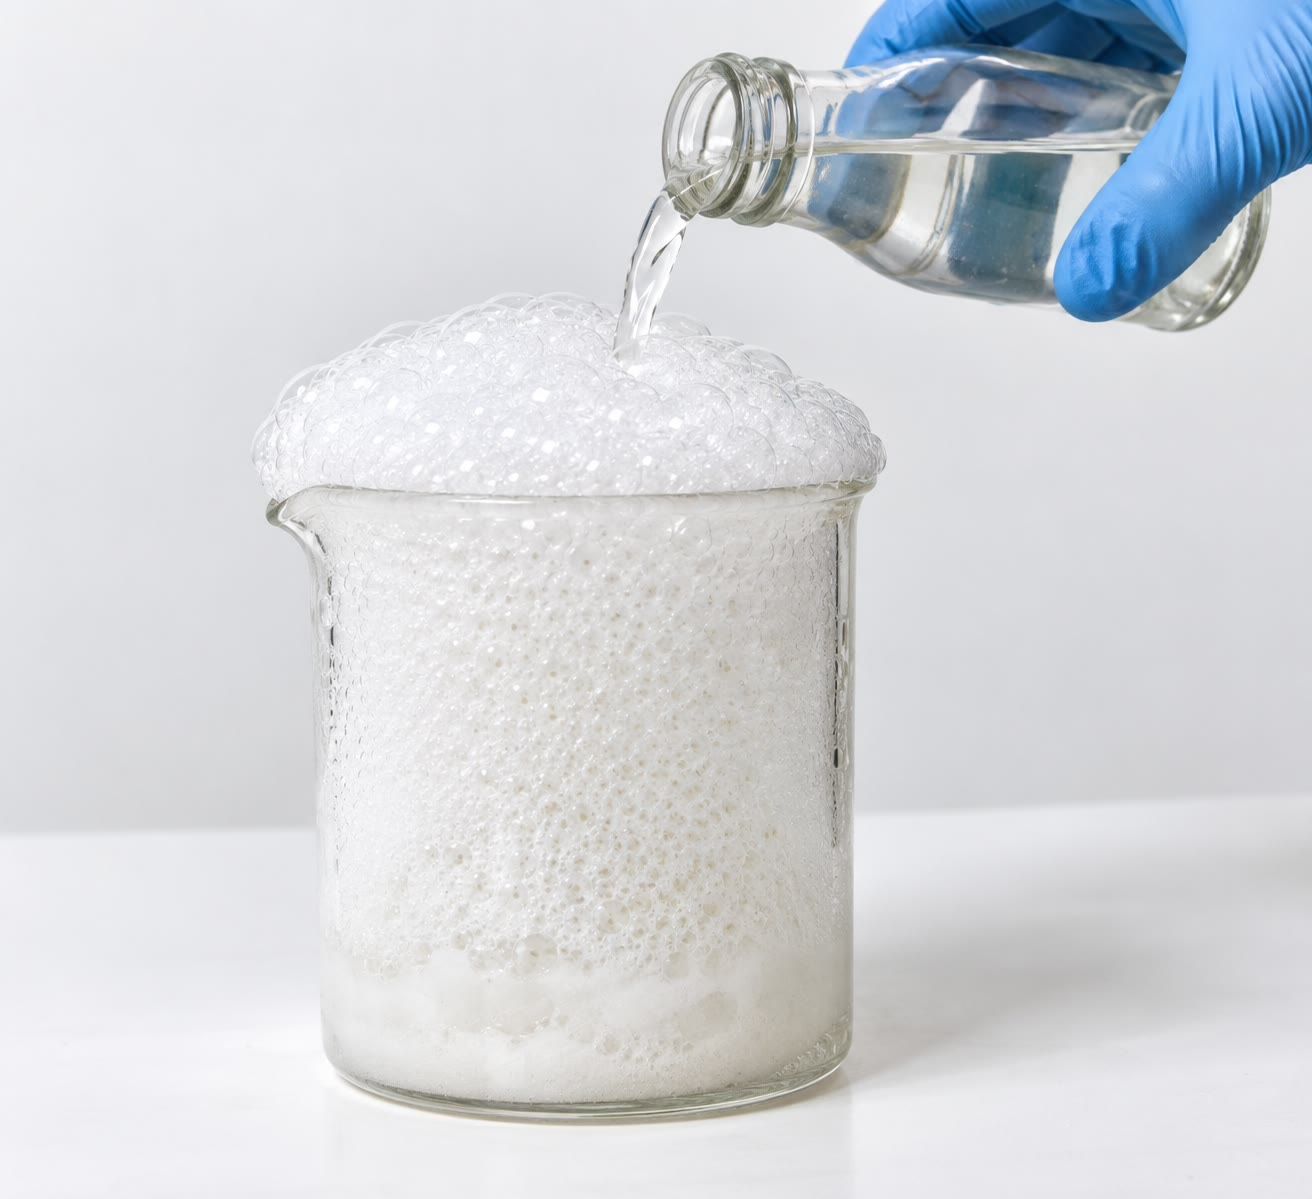
\includegraphics[width=0.5\linewidth]{images/book1/ai/g5-baking-soda-lab.jpg}

{\small Du vinaigre sur du bicarbonate de soude~: un gaz se dégage.}
\end{omfigure}

\section{Des transformations utiles et nuisibles}

\begin{proposition}[Les transformations chimiques autour de nous]\label{prop:g5:irreversible-changes:around}
Beaucoup de \omterm{def:g5:irreversible-changes:chemical-change}{transformations chimiques} sont utiles~: cuire les aliments,
faire du pain, \omterm{def:g4:what-a-fire-needs:burning}{brûler} du gaz pour chauffer une maison, le plâtre ou le
ciment qui durcissent en prenant. D'autres font des dégâts~: le fer qui
rouille, les aliments qui s'abîment, le bois qui pourrit. On ne peut pas
les défaire, mais on peut les ralentir~:
\begin{itemize}
  \item les aliments se conservent plus longtemps au froid du
        réfrigérateur~;
  \item la peinture ou un film d'huile protège le fer de l'\omterm{def:g4:air-a-mixture-of-gases:air}{air} et de
        l'eau~;
  \item une pomme coupée arrosée de jus de citron brunit plus lentement.
\end{itemize}
\end{proposition}

\begin{omfigure}
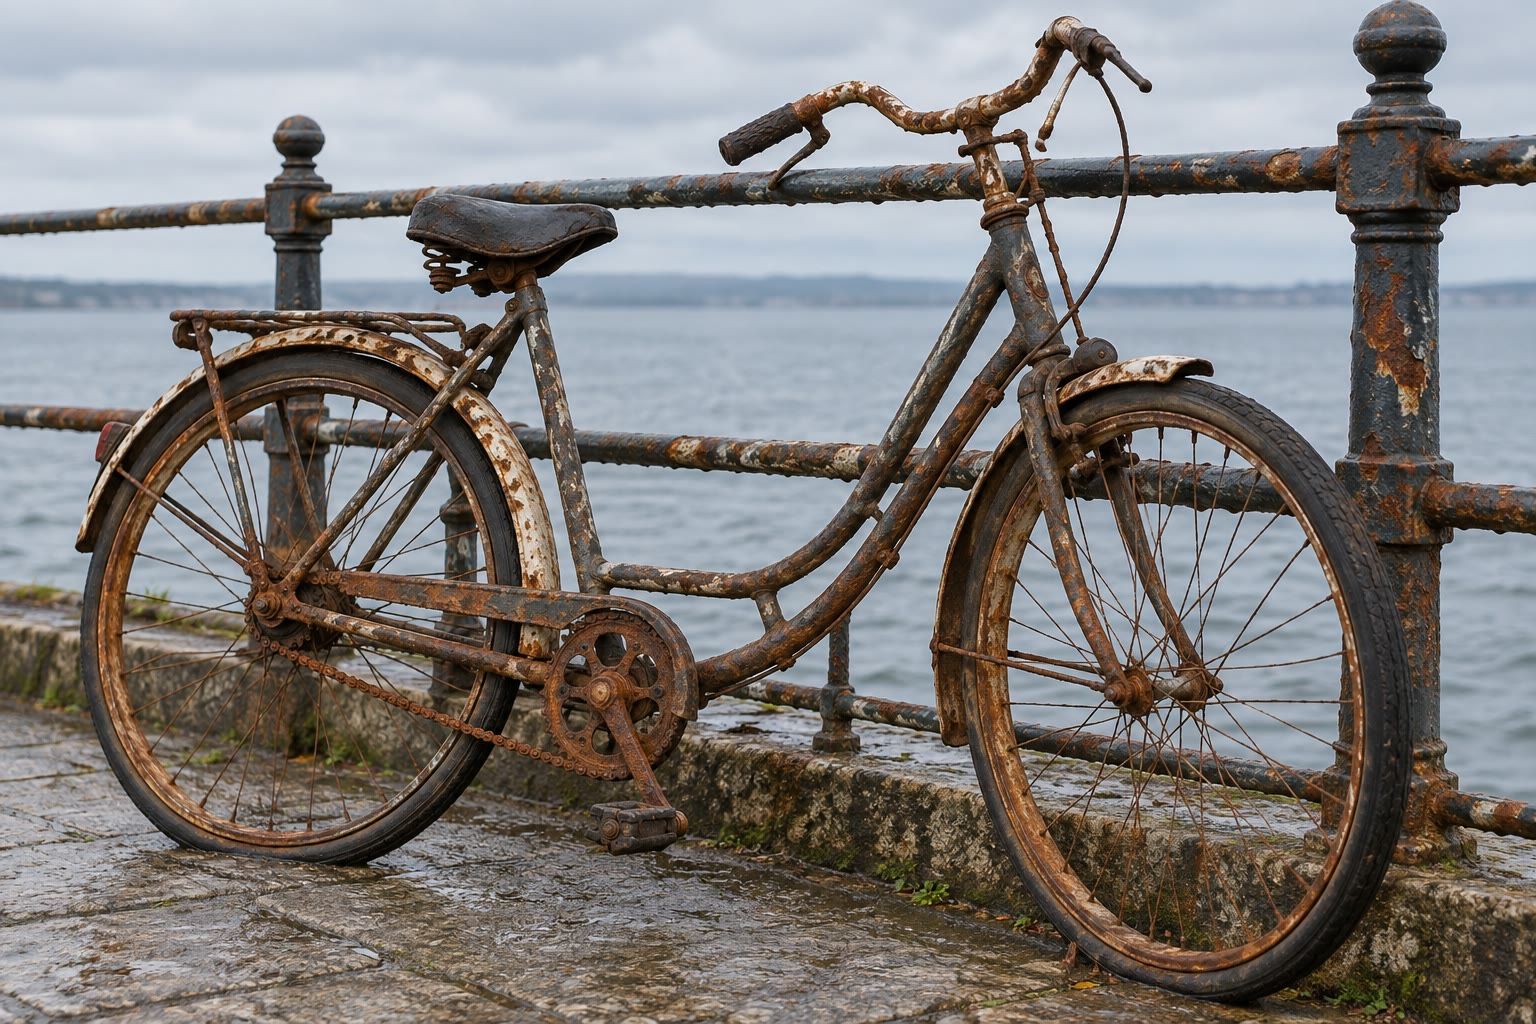
\includegraphics[width=0.55\linewidth]{images/book1/ai/g5-rusty-bicycle.jpg}

{\small Un vélo laissé des années sous la pluie~: le fer a rouillé.}
\end{omfigure}

\begin{remark}[Défaire, mais pas simplement]\label{rem:g5:irreversible-changes:not-simply}
«~Ne peut pas être défaite~» veut dire qu'il n'existe pas de chemin de
retour simple, comme refroidir ou faire sécher. Les chimistes savent
parfois retransformer la rouille en fer, mais seulement avec un haut
fourneau et de nouvelles substances~: c'est une autre \omterm{def:g5:irreversible-changes:chemical-change}{transformation
chimique}, pas un retour en arrière.
\end{remark}

\section{Exercices}

\begin{exercise}[$\star$]\label{exo:g5:irreversible-changes:1}
Dis si chaque transformation peut être défaite~: faire fondre du
chocolat, \omterm{def:g4:what-a-fire-needs:burning}{brûler} une allumette, dissoudre du sel dans l'eau, griller du
pain.
\end{exercise}

\begin{exercise}[$\star$]\label{exo:g5:irreversible-changes:2}
Qu'est-ce qu'une \omterm{def:g5:irreversible-changes:chemical-change}{transformation chimique}~? Donne deux exemples pris dans
la cuisine.
\end{exercise}

\begin{exercise}[$\star$]\label{exo:g5:irreversible-changes:3}
On dissout du sel dans l'eau. Comment peut-on récupérer le sel~? La
dissolution est-elle une \omterm{def:g5:irreversible-changes:reversible}{transformation réversible}~?
\end{exercise}

\begin{exercise}[$\star$]\label{exo:g5:irreversible-changes:4}
Quels indices d'une \omterm{def:g5:irreversible-changes:chemical-change}{transformation chimique} remarques-tu quand le lait
tourne~? Donnes-en deux.
\end{exercise}

\begin{exercise}[$\star$]\label{exo:g5:irreversible-changes:5}
Regarde la figure à deux colonnes. Quelles transformations ont une
double flèche~? Que signifie la double flèche~?
\end{exercise}

\begin{exercise}[$\star$]\label{exo:g5:irreversible-changes:6}
Pourquoi huile-t-on une chaîne de vélo~? Quelle \omterm{def:g5:irreversible-changes:chemical-change}{transformation chimique}
l'huile ralentit-elle~?
\end{exercise}

\begin{exercise}[$\star$]\label{exo:g5:irreversible-changes:7}
Quand on verse du vinaigre sur du bicarbonate de soude, ça pétille. De
quel indice s'agit-il~?
\end{exercise}

\begin{exercise}[$\star$]\label{exo:g5:irreversible-changes:8}
Nomme une \omterm{def:g5:irreversible-changes:chemical-change}{transformation chimique} utile et une \omterm{def:g5:irreversible-changes:chemical-change}{transformation chimique}
nuisible.
\end{exercise}

\begin{exercise}[$\star$]\label{exo:g5:irreversible-changes:9}
Pourquoi garde-t-on le lait au réfrigérateur~?
\end{exercise}

\begin{exercise}[$\star\star$]\label{exo:g5:irreversible-changes:10}
L'eau fait des bulles quand elle bout. L'ébullition est-elle une
\omterm{def:g5:irreversible-changes:chemical-change}{transformation chimique}~? Explique pourquoi un seul indice ne suffit
pas.
\end{exercise}

\begin{exercise}[$\star\star$]\label{exo:g5:irreversible-changes:11}
Tom dit~: «~Quand la bougie \omterm{def:g4:what-a-fire-needs:burning}{brûle}, la cire fond, tout simplement, comme
la glace.~» Utilise deux indices pour expliquer pourquoi la \omterm{def:g4:what-a-fire-needs:burning}{combustion}
d'une bougie est une \omterm{def:g5:irreversible-changes:chemical-change}{transformation chimique}, et pas seulement une
fusion.
\end{exercise}
